\documentclass[compress,11pt]{beamer}
%\includeonly{pendel}
\usetheme{Ilmenau}
%\usetheme{fau-4-3}
%\usecolortheme{beaver}
%\beamertemplatenavigationsymbolsempty
\usepackage[ngerman]{babel}
\usepackage{marvosym}
\usepackage{multimedia}
\usepackage[utf8]{inputenc}
\usepackage{amsmath}
\usepackage{amsfonts}
\usepackage{amssymb}
\usepackage{graphicx}
\usepackage{esvect}
%\author{}
\title{EP Gruppe 8}
%\setbeamercovered{transparent}
%\setbeamertemplate{navigation symbols}{}
%\logo{}
%\institute{}
%\date{}
%\subject{}
\usepackage{verbatim}
\begin{document}
\section{A4: Wandlerstrecke}
\begin{frame}
\begin{block}
Bisher: nur Betrachtung von D/A und A/D -Wandler einzeln\\
Nun: Aufbau einer Wandler-Strecke A/D-D/A:
\end{block}
Schaltung:\\
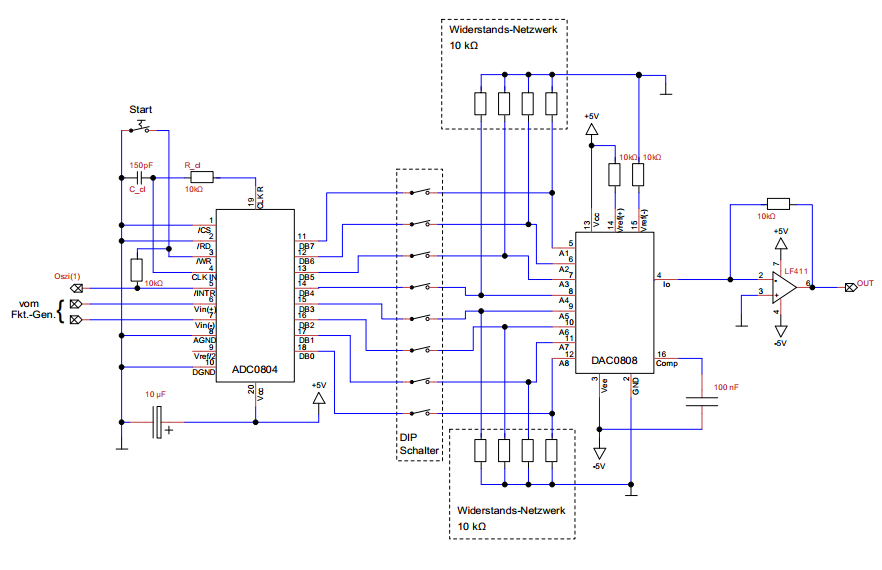
\includegraphics[width=.7\textwidth]{schalt41}\\
\tiny
Am Funktionsgenerator wurde im folgenden immer eine Spannung von $U_{pp} = 2 V$ mit $U_{offset} = 2 V$
\end{frame}
\begin{frame}
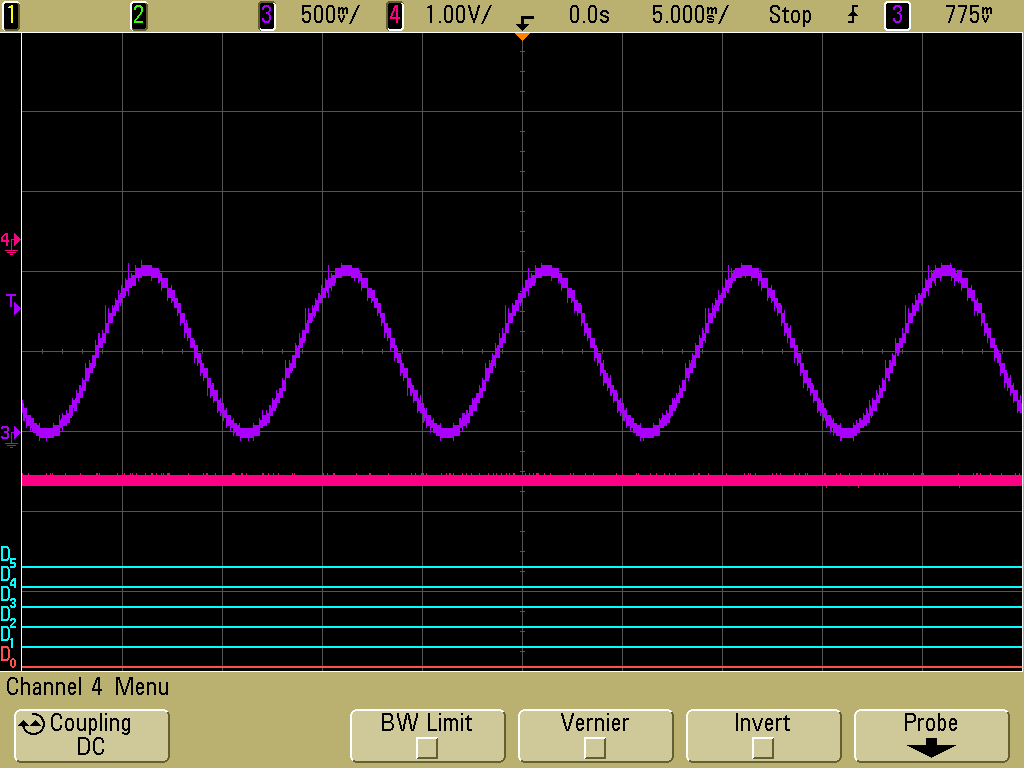
\includegraphics[width=.7\textwidth]{../vales_zeug/scope_128}\\
Funktionsweise wird hier ersichtlich: analoges Signal wird digitalisiert, um es dann wieder in ein analoges Signal umzuwandeln
\end{frame}
\begin{frame}
Mit folgender Apperatur am Ende der Schaltung kann das Signal hörbar gemacht werden:\\
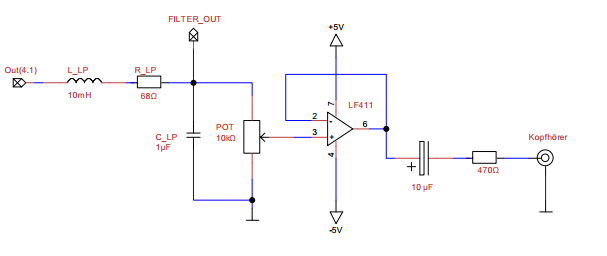
\includegraphics[width=.7\textwidth]{schalt42}\\
Zuerst war der Tiefpass durch Entfernung von C und Ersetzung von L mit einer Drahtbrücke iinaktiv\\
Nun wurden nach einander die einzelnen Schalter des Dip-Blocks abgeschaltet
\end{frame}
\begin{frame}
\begin{block}{Beobachtung}
\begin{itemize}
\item Alle Schalter eingeschaltet $\Rightarrow$ es ist eine Sinusschwingung mit Obertönen zu hören
\item Abschaltung der LSB $\rightarrow$ MSB  $\Rightarrow$ Obertonspektrum verschwindet, zum Schluss ist der Stromkreis komplett unterbrochen
\item  Abschaltung der MSB $\rightarrow$ LSB  $\Rightarrow$
Grundtöne verschwinden, Gesamtintensität dess Signals nimmt ab
\end{itemize}
Signifikanz des Bits $\backsim$ Beitrag der Intensität zum Ausgangssignal
\end{block}
\end{frame}
\begin{frame}
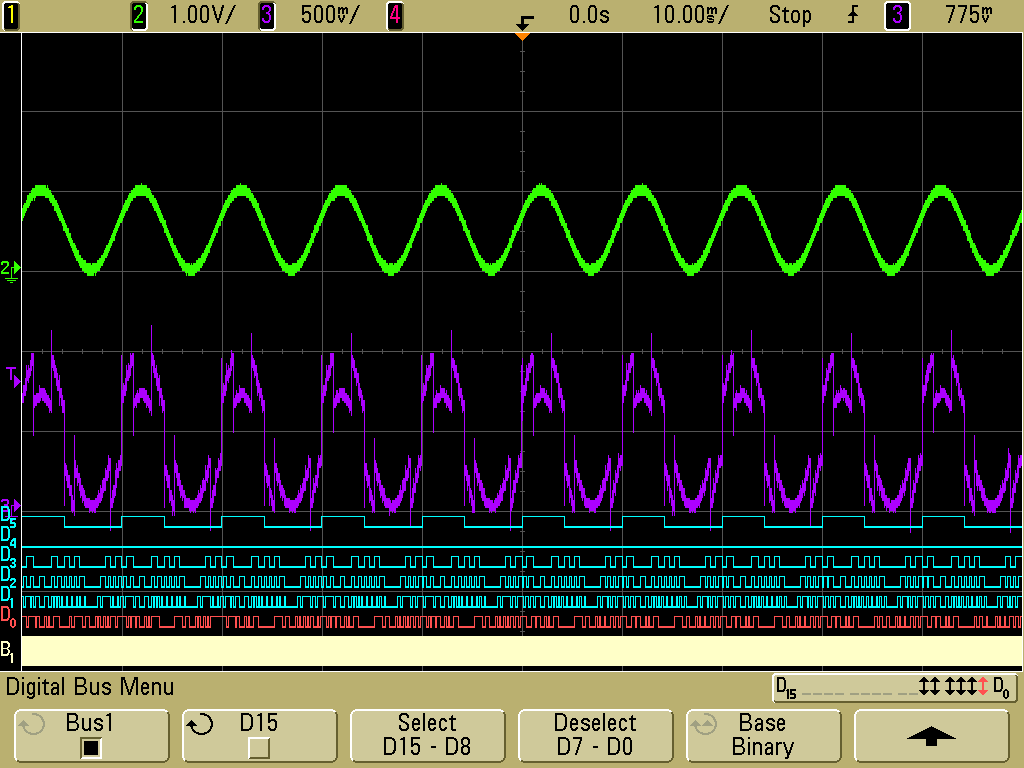
\includegraphics[width=.7\textwidth]{../vales_zeug/scope_132}\\
Ausgangssignal für die Schalterstellung 1110 1111 - Durch Entfernen dieses Bits kann das Signal nicht mehr vollständig übersetzt werden 
\end{frame}
\subsection{Shannon-Nynquist-Theorem}
\begin{frame}
Erhöhe nun die Frequenz des Eingangssignals:\\
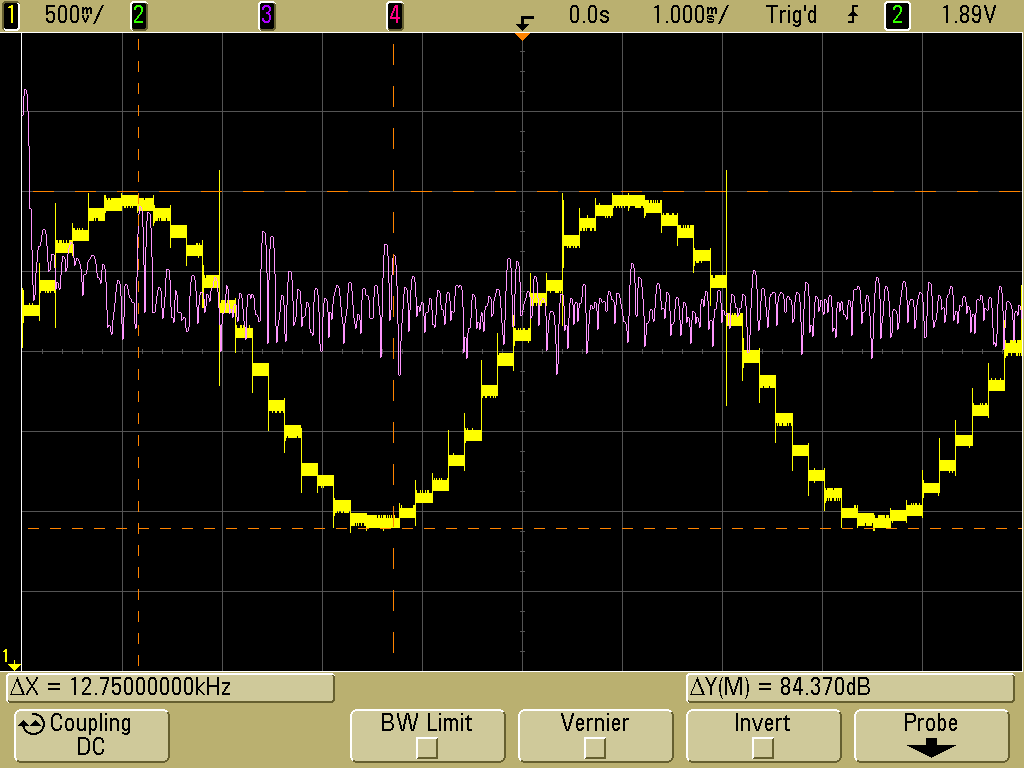
\includegraphics[width=.7\textwidth]{../scope_60}\\
$F = 200 Hz$
\end{frame}
\begin{frame}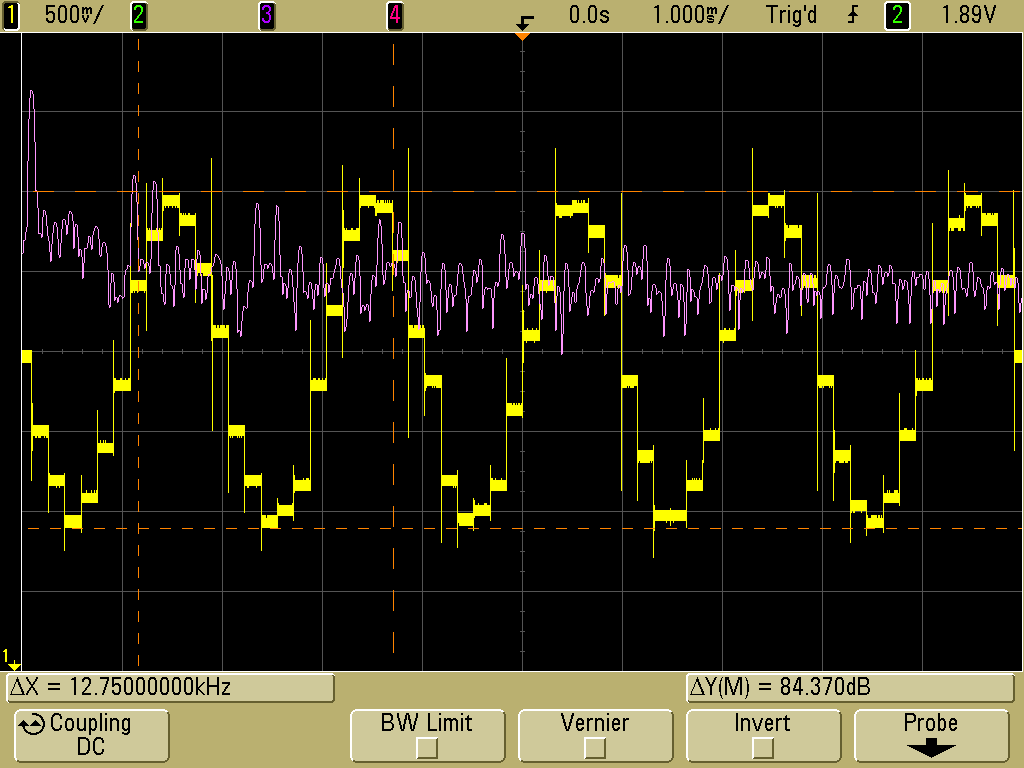
\includegraphics[width=.7\textwidth]{../scope_62}\\
$f = 500 Hz$
\end{frame}
\begin{frame}
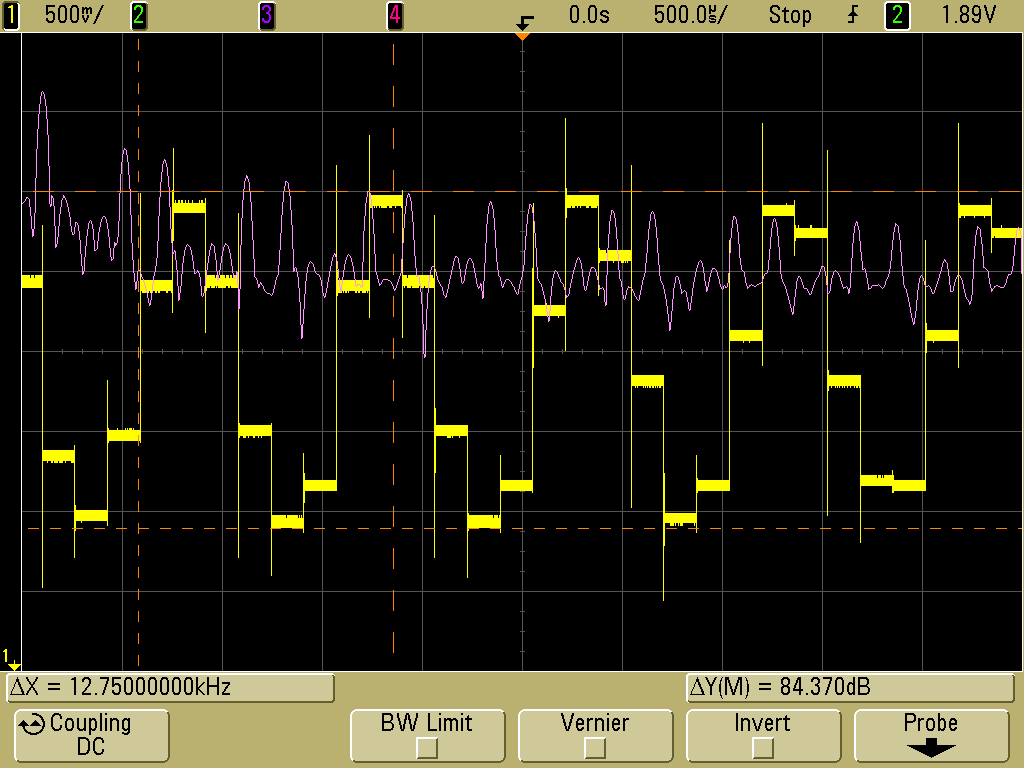
\includegraphics[width=.7\textwidth]{../scope_63}\\
$f = 1 kHz$
\end{frame}
\begin{frame}
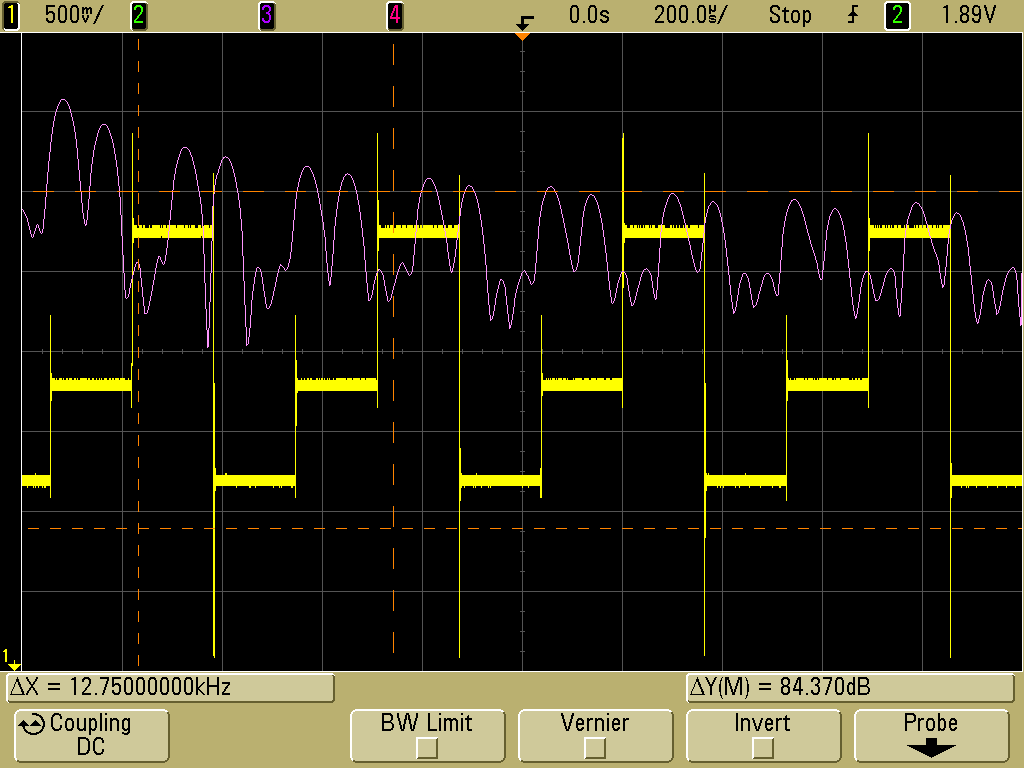
\includegraphics[width=.7\textwidth]{../scope_64}\\
$f = 2 kHz$
\end{frame}
\begin{frame}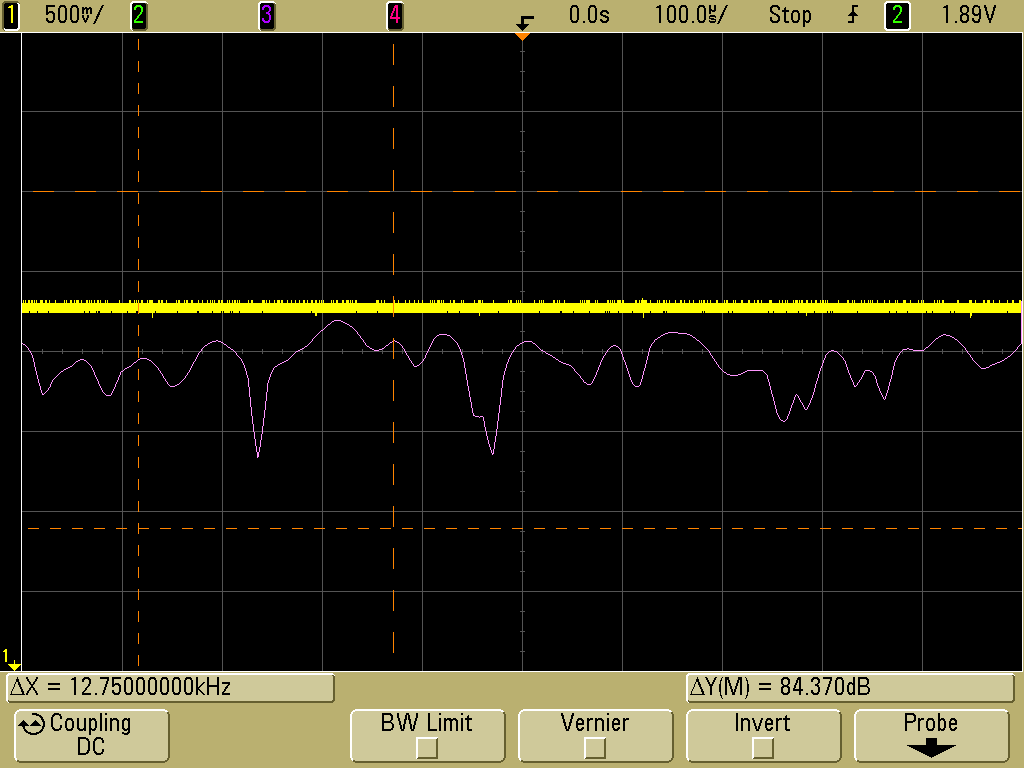
\includegraphics[width=.7\textwidth]{../scope_65}\\
$f = 4 kHz$
\end{frame}
\begin{frame}
\begin{block}{Beobachtungen}
\begin{itemize}
\item Je höher die Frequenz des Eingangssignals, desto ungenauer die Übersetzung, da das Signal ab einer best. Frequenz an zu wenigen Punkten abgetastet wird, um "angemessen" reproduziert zu werden
\item Akkustisches Signal wird mit zunehmender Frequenz verrauscht
\item führt auf Shannon-Nyquist-Theorem: bandbegrenzte Signale A(t) (also $F[A(t)] ( \omega ) = 0 $, für alle reellen $\omega$ ausserhalb eines Intervalls der Länge $f_{max} = 2 \cdot \pi \cdot \omega_{max}$ )
\end{itemize}
\end{block}
Da am FFT-Signal im Hintergrund ersichtlich ist, dass es sich hier nicht um ein bandbegrenztes Signal handelt - Filterung nötig, 
\end{frame}
\begin{frame}
Nun wird der bisher inaktive Frequenzfilter aktiviert: ebenso wird nun ein Ant-Aliasing-Filter vor die Apparatur geschaltet, um das weiter zu verwendende Signal im Frequenzraum auf ein Intervall zu beschränken (damit das Shannon-Nyquist-Theorem anwendbar ist)
\\

\end{frame}

\begin{frame}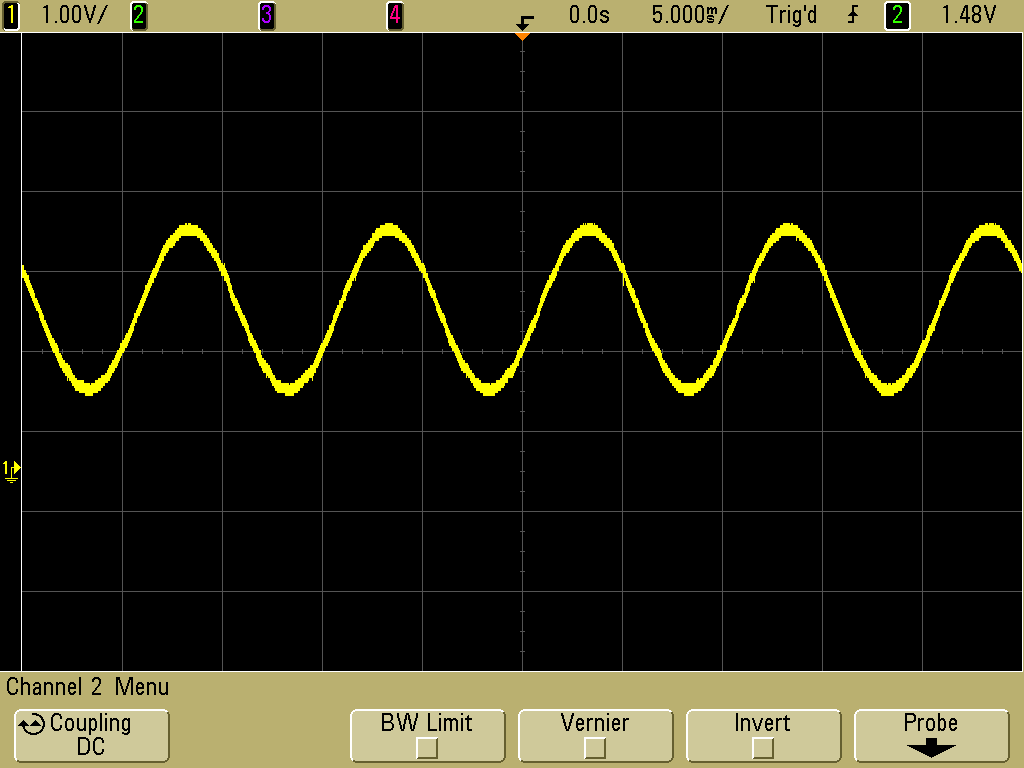
\includegraphics[width=.7\textwidth]{../scope_66}\\
$f = 4 kHz$
\end{frame}

\begin{frame}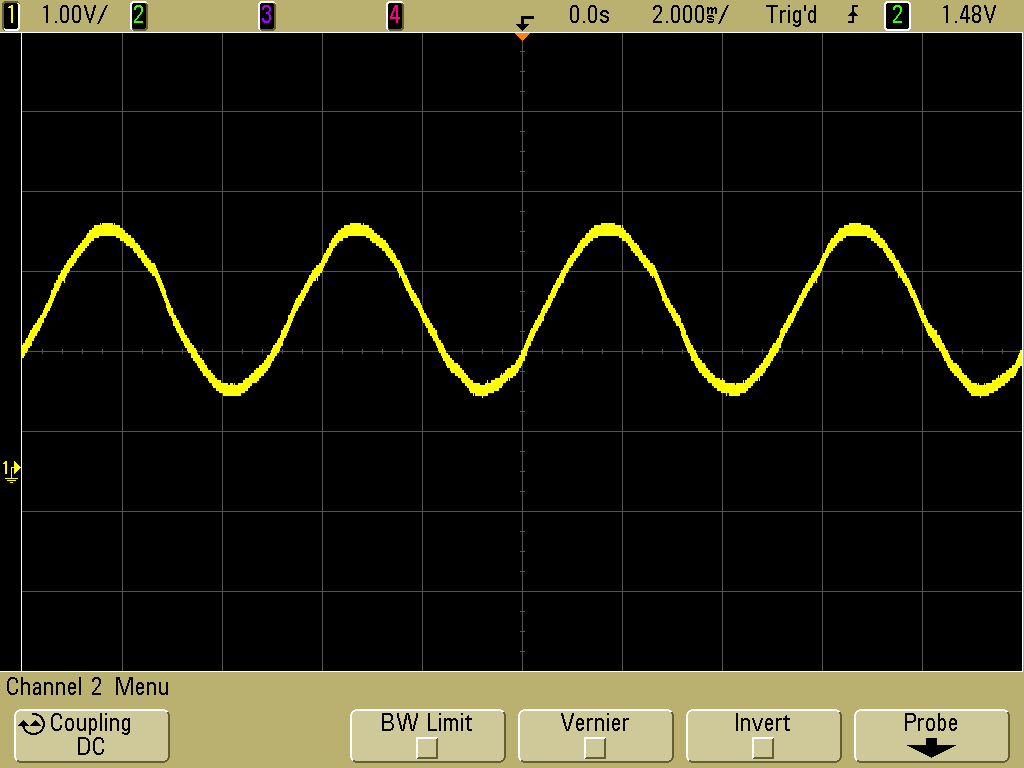
\includegraphics[width=.7\textwidth]{../scope_67}\\
$f = 4 kHz$
\end{frame}

\begin{frame}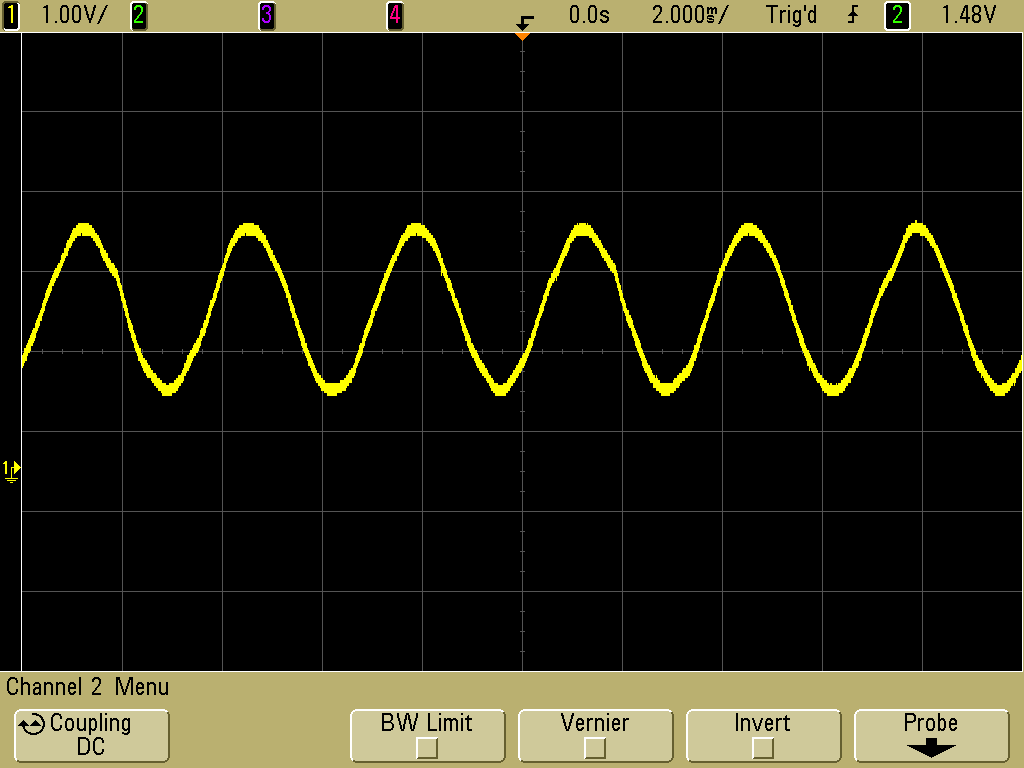
\includegraphics[width=.7\textwidth]{../scope_68}\\
$f = 4 kHz$
\end{frame}
\end{document}